
\chapter{Onderzoek: Tooling om analyses te doen op externe bibliotheken}
Bronnen:

\begin{itemize}
    \item https://medium.com/@manjula.aw/nodejs-security-tools-de0d0c937ec0
    \item
\end{itemize}
\begin{itemize}
    \item Javascript     https://github.com/RetireJS/retire.js
    \item SBT https://github.com/albuch/sbt-dependency-check
    \item
\end{itemize}
De eerste inzet om de opdracht tot een goed einde te brengen is het vinden van tooling om analyses te kunnen doen op externe bibliotheken. Voor nu is het zoeken naar een oplossing voor Scala en Typescript(Node.js) voldoende. In eerdere onderzoeken is naar boven gekomen dat de OWASP zich bezig houd met het veilig houden van geschreven software. Een van de projecten die de OWASp is "Dependency-check". Dit is een Software Composition Tool wat mogelijk maakt om openbaar gemaakte kwetsbaarheden te detecteren door te kijken of er voor dependencies een Common Platform Enumeration(CPE) bestaat. Als deze CPE bestaat kan er gekeken worden of er een CVE voor bestaat en vervolgens worden weergegeven in resultaten. Als geen van beiden bekend zijn wordt er door de tool vanuit gegaan dat er op het moment van checken geen kwetsbaarheid gevonden is. Hoewel dit op het oog een goede tool is om SOUP te analyseren is het in het project ontwikkelde versie niet mogelijk om te scannen op SBT en NPM dependencies. Op de website van het project is echter een link naar een versie die SBT projecten kan analyseren. En na een andere google search is een versie die voor NPM geschikt is ook gevonden.

In dit onderzoek worden deze twee tools getest om te achterhalen of deze tools daadwerkelijk geschikt zijn voor de doeleinden van het project. Dit wordt gedaan door de tools te gebruiken in een sandbox project die specifiek voor dit onderzoek is opgezet om de werking van de tool te achterhalen en vervolgens in een groot bestaand project om te kijken of de bevindingen in de sandbox ook te zien zijn in een echte situatie.
De onderzoeksvraag voor dit onderzoek luid dan ook: "Hoe zijn de gevonden tools te integreren in de methode om dependencies te analyseren en zijn de resultaten bruikbaar voor verder gebruik in de module?" Deze hoofdvraag geeft een aantal deelvragen die in de conclussie beantwoord dienen te zijn.
\begin{itemize}
    \item Hoe kan de tool worden gebruikt in huidige projecten?
    \item Komen de resultaten die gepubliseerd worden vanuit de projecten overeen met elkaar, Zijn de structuren vergelijkbaar?
    \item Wat doet de tool op de performance van de huidige Jenkins buildstraat, Hoelang heeft de tool nodig om resulaten te genereren?
    \item Zijn de resulaten voldoende om er daadwerkelijk een raport van te genereren die door de gebruikers gelezen kunnen worden.
    \item Hoeveel kennis van het project hebben de tools nodig om te functioneren? is de dependency declaratie voldoende of is het gehele project nodig voor de analyse.
\end{itemize}


\section{methode}
Om de bovenstaande deelvragen te beantwoorden is er gekozen om in drie situaties te testen. Iedere situatie wordt opgezet voor zowel de SBT(Scala) tools als die voor NPM(TypeScript).
\begin{enumerate}
    \item \textbf{sandbox omgeving} Dit is een omgeving waarbij een standaard project wordt opgezet met alleen de basis logica om het project te kunnen draaien. In het geval van Scala zal dit een playframework project zijn met daarin enkele database dependencies. Voor NPM zal dit een Angular Applicatie zijn met een UI framework.
    \item \textbf{Bestaand EagleScience Project}. Een project wat zowel een SBT-project bevat als een NPM(node.js) Project bevat.
    \item \textbf{ALleen de dependency declaraties} In het geval van SBT is dit dus de build.sbt en voor NPM is dit  een package.json en wellicht ook de package.json.lock.
\end{enumerate}

\section{Sandbox}
Het doel van deze test is om te kijken of de tooling überhaubt werkt en dat er bruikbare resultaten komen. De InteliJ wizards zijn gebruikt om een basis project op te zetten waar vervolgens volgens de documentatie de tooling is geimplementeerd.

Het resultaat is:

De gegenereerde JSON files zijn in opmaak identiek dus er kanmakkelijk een plugin geschreven worden die beide files in de database kan zetten
\section{}

https://github.com/etnetera/owasp-dependency-check for Node.js /NPM
https://github.com/albuch/sbt-dependency-check for SBT


Dit hoofdstuk geeft het onderzoek weer naar tools die binnen EagleScience ingezet kunnen worden voor het analyseren van de dependencies. De hoofdvraag in dit onderzoek is dan ook: "Welke tools kunnen er ingezet worden om binnen de dev-stack van EagleScience een analyse te doen op kwetsbaarheden in externe biblotheken?" Om deze vraag te kunnen beantwoorden zijn de volgende deelvragen opgesteld die samen een conclussie opleveren die gebruikt kan worden in het ontwerp van de module.

De deelvragen opgesteld voor dit onderzoek zijn:\\
\begin{itemize}
    \item Welke tools bestaan er om dependency informatie uit een sbt en npm project te halen?
    \item Hoe zijn de tools in te zetten in de huidige projecten?
    \item Welke output wordt er verkregen van de tools?
    \item Is er de mogelijkheid om geautomatiseerd data uit deze tools te halen om deze vervolgens te kunnen weergeven.
\end{itemize}

\section{Bronnen voor dit onderzoek}
https://www.softwaretestinghelp.com/tools/top-40-static-code-analysis-tools/
\section{Welke tools bestaan er on dependency analyses uit te voeren op dev-stack van Eaglescience.}\label{sec:welke-tools-bestaan-er-on-dependency-analyses-uit-te-voeren-op-dev-stack-van-eaglescience.}
Er zijn verschillende tools beschikbaar die helpen om applicaties veiliger en/of beter te maken. De tools kunnen worden opgedeeld in twee categoriën aan de ene kant zijn er tool suites die beloven dat door goed gebruik te maken van deze tools de software die uitgerold beter en veiliger wordt. Deze tools kijken veelal naar de opbouw van geschreven sourcecode en het gebruik van externe bibliotheken. Een aantal bekende voorbeelden zijn: "Sonarqube", "embold", "Snyk.io". Hoewel veel van deze tools veel ontwikkeltalen kan onderzoeken, missen de meeste ondersteuning voor Scala. Wat op dit moment de go-to taal is van EagleScience. Als er al ondersteuning is wordt dit meestal middels een comunity plugin geintroduceerd. Een andere aspect is dat veel van deze toolsuite een lictentie nodig hebben om alle onderdelen te kunnen gebruiken. De manier waarop deze toolsuites werken is dat er een snapshot wordt gemaakt van een repo waar vervolgens een analyse op gedaan wordt.

Een andere vorm van tooling is tooling dat ingebouwd kan worden in bestaande pipelines. Veel aanbieders van Source control systemen die ook een mogelijkheid hebben om een CI-CD pipe line te bouwen op deze structuren bieden mogelijkheden om analyses te doen op source-code. Een enkele voorbeelden zijn Github, GitLab en Bitbucket. Ook al maakt eaglescience gebruik van gitlab deze vorm van analyseren in gitlab gaat niet werken gezien Eaglescience deze alleen gebruikt voor version control. Als CI-CD pipeline wordt op het moment de automatiserings server Jenkins gebruikt.

Vanuit EagleScience is aangegeven dat de huidige pipeline niet of zo weinig mogelijk aangepast mag worden. En dat een nieuwe toolsuite op het moment niet in de budgetering past. Er moet dus gezocht worden naar een "open source" oplossing die binnen Jenkins past. Door deze restricties is het dus niet mogelijk om een toolsuite te gaan gebruiken. Een optie is om zelf middels andere tooling welke voor in het geval van EagleScience geschikt is voor het analyseren van Scala(SBT) en Typescript(Node.js/NPM) te vinden en deze te integreren in Jenkins. Om vervolgens zelf de resultaten te publiseren in de portal.


\section{Tooling voor de door EagleScience gebruikte buildtools, SBT en NPM}
Gezien tool suites niet de juiste oplossing zijn moet er gezocht worden naar een manier om alsnog de analyse uit te kunnen voeren. Eén van de belangrijkste schakels om dit te kunnen doen is de analyse van de dependency files binnen de projecten. Zoals eerder onderzocht zijn er drie belangrijke onderdelen binnen de dev stack waarop gecontroleerd dient te worden: SBT voor Scala backend projecten en NPM voor de node.js 'frontend' projecten. Als we de dev\-stack systematisch van gebruiker naar platform aflopen is eerst NPM aan de beurt en vervolgens SBT. Zoals in het vorige onderzoek naar boven is gekomen heeft de OWASP als doel software veiliger te maken. Te lezen was dat ze dit deels doen door awareness middels de top-10 en symposia te houden. Echter zijn er ook proactievere projecten binnen OWASP, zoals de ontwikkeling van een dependency check. (https://owasp.org/www-project-dependency-check/). Deze dependency check is geschikt voor de meest voorkomende talen die gebruikt worden, echter is Scala niet veel gebruikt en wordt dus niet direct ondersteunt. Verder onderzoek binnen het project geeft weer dat het voor Node projecten wel ondersteuning bied middels de NPM -audit tool die al in NPM ingebouwd is op dependencies te scannen. Dit project lijkt dus niet voor de hand liggend om te gebruken. Maar bied wel mogelijkheden om als startpunt te gebruiken.

Binnen de OWASP bestaat er een werkgroep die zich bezig houden met het scannen van kwetbaarheden in dependencies: https://owasp.org/www-project-dependency-check/  De OWASP is als uitgangspunt genomen voor het zoeken naar tooling die gebruikt kan worden voor het analyseren van de projecten.


\subsection{NPM}\label{subsec:npm}
Als de OWASP Dependency check documentatie na wordt gelezen bestaat er geen directe module voor het checken van NPM packages. (https://jeremylong.github.io/DependencyCheck/analyzers/index.html). Er wordt zelfs aangegeven dat het gebruik maakt van een tool ingebouwd in NPM genaamd NPM-audit.
Uit de documentatie van deze tool is het in staat om alle dependencies die in de package.json en de package-lock.json te kunnen nagaan op kwetsbaarheden zonder dat een project daadwerkelijk gebouwd hoeft te worden. Het is dus in staat om kwetsbaarheden te vinden zonder dat er source-code wordt doorzocht.
Dit heeft zowel voor als nadelen. Een voordeel is de tijd die het duurt om een analyse uit te voeren. gezien het niet gebouwd hoeft te worden zal er geen tijd worden opgeslokt voor een build die mogelijk niet gebruikt kan worden. Een nadeel zou kunnen zijn dat een analyse op alleen de dependencies en het gebruik ervan buiten beschouwing laten wellicht keuzes voorschotelen voor updates die wellicht helemaal niet nodig zijn omdat de kwetsbare code toch niet gebruikt wordt. Door gebruik te maken van "NPM -audit" worden de translative packages ook meegenomen en daarmee dus ook inzichtelijk. In veel gevallen wordt er zelf een remedie genoemd om de kwetsbaarheid te verhelpen zoals te zien is in figuur~\ref{fig:npmauditresult}
\begin{figure}[H]
    \centering
    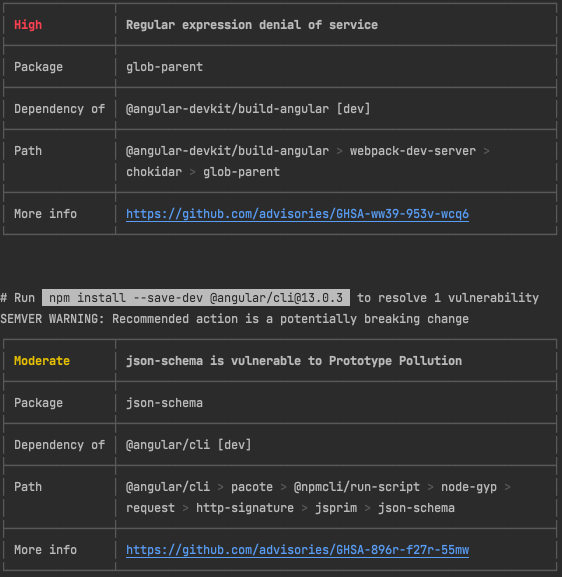
\includegraphics[width=10cm]{gfx/Screenshot NPM audit}
    \caption{Screenshot NPM audit result}
    \label{fig:npmauditresult}
\end{figure}


\subsection{SBT}\label{subsec:sbt}
Voor het analyseren van sbt projecten zijn meerdere manier. Veelal zijn dit checks die in bestaande CI-CD pipeline van bijv. GitLab, GitHub(CircleCI) worden betrokken. Een voorbeeld hiervan is een tool dat gebruik maakt van Gemnasium als analyse tool. Echter is het overhevelen van de pipeline naar Gitlab op dit moment geen optie gezien er een requirement bestaat dat de huidige pipeline moet blijven bestaan met minimale aanpassingen. De volgende optie zou zijn om een plug-in voor Jenkins te gebruiken, welke bestaat, echter is hier het probleem dat deze voor adoptie is aangeboden en er dus de kans bestaat dat de support en ontwikkeling stil komt te liggen. Deze zijn geen optie voor EagleScience omdat dit zou betekenen dat de huidige pipeline zou moeten verhuizen van de bestaande Jenkins naar een pipline aangeboden door GitLab. Welke we al gebruiken als Repository voor de geschreven code. Om toch gebruik te kunnen maken van Jenkins zou de eerst volgende optie zijn om gebruik te maken van een plugin die de check uitvoerd. Er bestaat de OWASP-dependency-check plug die analyseert of er kwetsbaarheden bestaan in een project er zijn Een voordeel zou kunnen zijn dat er quality gates toegevoegd kunnen worden aan de plugin zodat deze de build kan stoppen op het moment dat er kwetsbaarheden gevonden zijn die boven een theshold liggen. Daarnaast zijn er twee nadelen 1: De plugin wordt op het moment van schrijven ter adoptie aangeboden op de Jenkins plugins pagina. En de output die het genereerd is een XML-format. En gezien JSON makkelijker te verwerken is richting een mongodb en het feit dat de NPM als enige optie een JSON-output geeft. Is er nog een laatste optie en dat is een plug-in in het sbt project wat in staat steld om binnen een project een analyse te doen. De voordelen zijn als eerste dat deze een JSON-output geeft. Heeft de mogelijheid om ingezette worden in een pipeline door het stellen van een CVSS score theshold dat de build doet falen op hetm moment dat deze waarde wordt overschreven. (dan moet de SBT plugin wel aangeroepen worden binnen de pipeline). De sbt plugin geeft ooutpu in veschillende formats en niet onbelangrijk JSON waarmee het potentieel makkelijk te integreren is met de resultaten die uit de NPM audit komen.


\section{Methoden om vanuit de Jenkins pipeline SOUP-analyse resultaten te verkrijgen}\label{sec:methoden-om-vanuit-de-jenkins-pipeline-soup-analyse-resultaten-te-verkrijgen}
Nu we methodes hebben voor het verkrijgen van SOUP-analyse resultaten. Moet er onderzocht worden wanneer we deze analyse uitvoeren. In feite zijn er in dit geval twee opties.
\begin{enumerate}
    \item Er wordt een analyse uitgevoerd als onderdeel van de buildpipeline binnen Jenkins
    \begin{itemize}
        \item voordelen:
        \begin{itemize}
            \item alles is geintegreerd in een enkele omgeving.
        \end{itemize}
        \item nadelen:
        \begin{itemize}
            \item Build tijden kunnen langer gaan duren.
            \item moet een plugin/script komen die resultaten maakt die door de module kan worden ingelezen en weergegeven.
        \end{itemize}
    \end{itemize}
    \item of er wordt informatie over de dependencies verstuurd naar een aparte module welke daar wordt geanalyseerd
    \begin{itemize}
        \item voordelen:
        \begin{itemize}
            \item Build tijden lopen niet op omdat analyse niet in de pipeline gedaan wordt.
            \item alleen de data van de dependencies dienen te worden verstuurd Rapportage wordt gedaan door de module.
            \item
        \end{itemize}
        \item nadelen:
        \begin{itemize}
            \item resultaten zijn later beschikbaar dan de deploy gedaan is.
            \item
        \end{itemize}
    \end{itemize}
\end{enumerate}

\section{Conclusie}\label{sec:conclusie}
Er zijn door restricties vanuit eaglescience twee potentiele candidaten die dependency informatie kunnen verkrijgen en daar een analyse op kunnen doen:

voor SBT is dit sbt-depenency-check geschreven door Alexander v. BuchHoltz(Albuch op Github)
En voor het scannen van NPM packages bestaat er al een tool binnen NPM die ook output kan leveren.

In het onderzoek beschreven in het volgende hoofdstuk zal worden onderzocht of deze twee tools daadwerkelijk de gewenste output geven. En zal er worden onderzocht hoe deze tools de gewenste resultaten kan opleveren.
